\documentclass[a4paper,11pt]{article}

\usepackage{cmap}		
%\usepackage[utf8]{inputenc}			
\usepackage[brazil]{babel}
\usepackage{framed}
\usepackage{hyperref}
\usepackage{amsmath}
\usepackage{graphicx}
\usepackage[colorinlistoftodos]{todonotes}
\usepackage{wrapfig}
\usepackage{lipsum}
\usepackage{listings}
\usepackage{color}
\usepackage{indentfirst}
\usepackage{times}
\usepackage{textcomp}
\usepackage{pgfgantt}
\usepackage{lipsum}

% set document font, font sizes, margin dimensions and spacing
\usepackage{fontspec}
\setmainfont{Arial}
\usepackage[top=15mm,bottom=25mm,left=20mm,right=20mm]{geometry}
\usepackage{setspace}\onehalfspacing
\usepackage{titlesec}
\titleformat*{\section}{\Large\bfseries}
\titleformat*{\subsection}{\Large\bfseries}
\titleformat*{\subsubsection}{\Large\bfseries}
\titleformat*{\paragraph}{\Large\bfseries}
\titleformat*{\subparagraph}{\Large\bfseries}
\setlength{\parskip}{0.6em}

\newif\ifblackandwhite
\blackandwhitetrue

\usepackage{etoolbox}
\usepackage{longtable}%
\AtBeginEnvironment{longtable}{%
  \addfontfeature{RawFeature=+tnum;-onum}%  <--- requires LuaTeX
}

\usepackage{pdflscape}
%\usepackage[svgnames]{xcolor}
 \usepackage{colortbl}%
   \newcommand{\myrowcolour}{\rowcolor[gray]{0.925}}
\usepackage{booktabs}

\ifblackandwhite
  \newcommand{\cheading}[2]{\textbf{#1\hfill #2}}
  \newcommand{\highest}[1]{\textbf{#1}}% == highest score for question
\else
  \newcommand{\cheading}[2]{\textcolor{Maroon}{\textbf{#1\hfill #2}}}
  \newcommand{\highest}[1]{\textcolor{Maroon}{\textbf{#1}}}%
\fi

\definecolor{mygray}{rgb}{0.4,0.4,0.4}
\definecolor{mygreen}{rgb}{0,0.8,0.6}
\definecolor{myorange}{rgb}{1.0,0.4,0}

\setcounter{secnumdepth}{5}
\setcounter{tocdepth}{4}

\lstdefinestyle{customc}{
  belowcaptionskip=1\baselineskip,
  breaklines=true,
  frame=L,
  xleftmargin=\parindent,
  language=C,
  showstringspaces=false,
  basicstyle=\footnotesize\ttfamily,
  keywordstyle=\bfseries\color{green!40!black},
  commentstyle=\itshape\color{purple!40!black},
  identifierstyle=\color{blue},
  stringstyle=\color{orange},
  numbers=left,
  numbersep=12pt,
  numberstyle=\small\color{mygray},
}
\lstset{escapechar=@,style=customc}

\newcommand{\HRule}{\rule{\linewidth}{0.5mm}}

%Definindo um comando todoin que aceita quebra de linha e fórmulas
\newcommand\todoin[2][]{\todo[inline, caption={2do}, #1]{
\begin{minipage}{\textwidth-4pt}#2\end{minipage}}}

\newcommand\todogeg[2][]{\todo[inline, caption={#2}, color=yellow!100, #1]{
\begin{minipage}{\textwidth-4pt}#2\end{minipage}}}

\newcommand\todovwcm[2][]{\todo[inline, caption={#2}, color=red!100, #1]{
\begin{minipage}{\textwidth-4pt}#2\end{minipage}}}

\begin{document}

\begin{titlepage}
    \begin{center}

        % logo
        
\includegraphics[width=0.15\textwidth]{images/ufsc_logo_sf.png}~
        \\[2cm]

        \textsc{\large <Título do Plano de Trabalho do Aluno>(Aqui escreve MIGMASTATS?)}
        \\[2cm]

        % identificação do relatório
        \HRule \\[0.4cm]
        {\large \bfseries Relatório Final das atividades do Programa Institucional \\
        de Bolsas de Iniciação Científica e Voluntário PIBIC \\
        Edital 2021\\[0.4cm]}
        \HRule
        \\[2cm]

        % identificação do aluno
        \large\textbf{Aluno}\\
        Rodrigo Ferraz Souza\\
        Engenharia de Computação \\
        Programa PIBIC
        \\[1cm]

        % identificação do orientador
        \large\textbf{Orientador}\\
        Antônio Carlos Sobieranski\\
        <Departamento/Unidade Acadêmica> (não sei o que é isso)
        \\[1cm]

        % identificação do projeto de pesquisa
        \large\textbf{Projeto de Pesquisa}\\
        Análise Estatística do Dataset MIGMA (ver depois no doc que eu assinei)\\[1cm]


        \vfill

        % Bottom of the page
        {\large \today}

    \end{center}
\end{titlepage}

\newpage
\begin{abstract}
  no máximo 1 página

\end{abstract}

\newpage
\tableofcontents
\newpage
\section{Introdução}
\label{sec:introducao}

Exemplo de referência para figura

Como visto na Figura~\ref{fig:lifecycle_phase} $\ldots$

\begin{figure}[ht]
    \center
    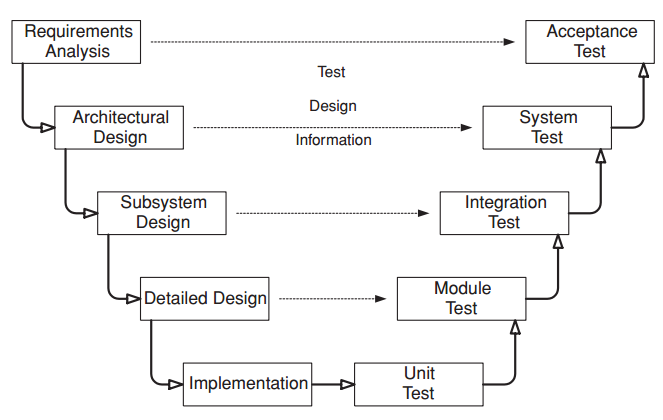
\includegraphics[scale=0.7]{images/lifecycle_phase.png}
    \caption{Testing levels based on software development phase (Sommerville, 2011).}
    \label{fig:lifecycle_phase}
\end{figure}

Exemplo de referência para bibliografia

De acordo com \cite{sommerville2011software} $\ldots$

\section{Objetivos}
\label{sec:objetivos}

Descrever o objetivo geral. Elencar e explicar cada um dos objetivos específicos.

\textbf{Objetivos específicos}

\begin{itemize}
    \item Objetivo específico 1 : 
    \item Objetivo específico 2 : 
\end{itemize}

\section{Materiais e Métodos}
\label{sec:materiais}

Descrever aqui o que foi feito durante o projeto e colocar o fluxograma.
Todo o projeto foi desenvolvido e documentado no Github (colocar o link)

\subsection{Correlação com os múculos da Face}
Aqui foi tentado fazer algumas correlações com os músculos faciais, contudo, ao que foi descoberto no item ?? sobre a analise de exprsssões em vídeos e a alta complexidade dos músculos, foi abandonada esta estratégia e optado por fazer a redução dos dados para otimizar a análise utilizando agrupamento por KMeans descrito no item ??.

\subsection{Experimentos}
\subsubsection{Experimento 1 - Analise dos rostos e coleta dos dados de LandMarks}
O objetivo é coletar os dados para que possam ser analisados e correlacionados posteriormente.

Foi analisada cada imagem de cada pessoa em cada uma das expressões e o resultado será salvo na pasta processed da seguinte forma.
\begin{verbatim}
.
├── /processed
|   |
|   ├── [id_expressão]
|   |   |
|   |   ├── mean_[id_expressão].png (Mascara com triangulos fantas da expressão com fundo branco)
|   |   ├── [id_supervisionado]
|   |   |   ├── [id_pessoa]
|   |   |   |   |
|   |   |   |   ├── [id_foto].csv (vai conter as posições xy dos landmarks da foto)
|   |   |   |   ├── [id_foto].jpg (Mascara de triangulos da pessoa com fundo preto pra cada foto)
|   |   |   |   ├── mean_[id_pessoa].jpg (Mascara de triangulos fantasma da pessoa com fundo branco)

\end{verbatim}

\paragraph{Descrição dos Arquivos}
\begin{itemize}
    \item{analyser.py}
    \subitem{Anda de pasta em pasta do dataset e salva os .csv em processed na pasta raiz do projeto}

    \item{draw\_triangles.py}
    \subitem{Anda pelas pastas de processed e, a partir dos csv, gera as mascaras e as salva em .jpg no mesmo diretório}

    \item{error\_verifier.py}
    \subitem{Verifica e exclui as inconsistencias encontradas no dataset, como pastas com numeros equivocados de imagens, e casos nos quais faces não foram reconhecidas}

    \item{face\_mesh.py}
    \subitem{Uma classe para extrair os pontos da face}

    \item{face\_adjustments.py}
    \subitem{Faz as transformações na imagem a partir dos pontos extraidos, de acordo com as definições abaixo}

\end{itemize}

\paragraph{Procedimentos}\mbox{}\\



Para melhor analisar as imagens posteriormente um padrão será adotado, e ele será o seguinte:
\begin{itemize}
    \item{Todas as imagens serão rotacionadas para que os olhos fiquem sempre na mesma linha (alignEyes)}
    \item{O ponto 10 é deixado sempre na altura 25 e no centro da imagem, com a distancia entre o ponto 10 e o ponto 152 sendo de 1500px (alignFace)}
    \subitem{Colocar aqui uma imagem com as linhas mostrando o tamanho do rosto sendo 1500px}
    \item{A imagem será recortada em um retangulo, deixando apenas o rosto centralizado, com margem de 25px.}
    \item{A imagem será deixada com 1900px X 2500px sem redimensionar, apenas colocando bordas pretas nas laterais e em baixo para completar o tamanho}
    \item{somente então será salva com os dados relativos a imagem no fim deste processo}
\end{itemize}
Colocar aqui o bloco do experimento 1 do fluxograma


\paragraph{Remoções do Dataset Neste Experimento}\mbox{}\\
\subparagraph{Motivo: Número incorreto de fotos em uma pasta do usuário}\mbox{}\\
nos casos em que foi detectado que uma das pastas do usuário continha um numero diferente de 3 fotos, todas as pastas dele foram removidas da analise. Os usuários que esta regra foi aplicada são os que seguem, com as seguintes observações:
\begin{itemize}
    \item{00541 - 4 imagens em 00/00}
    \item{02069 - 11 imagens em 00/00}
    \item{05669 - 7 imagens em 00/00}
    \item{06644 - 2 imagens em 00/00}
\end{itemize}

\paragraph{Exemplo de Máscara gerada com os Landmarks obtidos}\mbox{}\\
colocar a imagem aqui da mascara com o fundo preto

\paragraph{Vídeo das Faces e Máscaras}\mbox{}\\
Fui obrigado a colocar o video no drive pois ele acabou ficando ridiculamente pesado (cerca de 4,5gb) O codec utilizado não é suportado pelo reprodutor do windows, abra o video com o VLC que irá ser lido normalmente. O as imagens utilizadas no video tem 1/3 de seu tamanho original, para reduzir o tamanho do mesmo. Deixando-o com a resolução de 1666x633 px
(colocar o link pro vídeo ou um print dele sla)
No video as informações estão dispostas da seguinte forma:

\begin{itemize}
    \item{Na esquerda está o rosto cortado da pessoa}
    \item{Na direita a máscara extraida deste rosto}
    \item{no meio estão o tipo/expressão (ids) e o id da pessoa, respectivamente}
    \item{a cada troca de pasta (tipo ou expressão) é mostrado por 2s uma imagem do novo diretorio com os ids (tipo/expressão)}
\end{itemize}


\subsubsection{Experimento 2 - Processamentos dos Dados Obtidos no Experimento 1}
O objetivo aqui é tentar encontrar um padrão para os dados obtidos no experimento 1, e fazer um processamento dos dados para que possam ser utilizados no experimento 3.

\paragraph{Primeira Abordagem - Todos os Pontos (Foi abandonada)}\mbox{}\\
\subparagraph{Parte 1}\mbox{}\\
Para cada uma das máscaras de um usuário, obter as distâncias de cada ponto desta máscara para sua mascára neutra não supervisionada (00/00). Com esses dados, também gerar distâncias médias para a neutra NS de todos os usuários

\subparagraph{Parte 2}\mbox{}\\
A partir dos dados gerados na parte 1, que são MUITOS, reduzílos a alguns números que, em teoria, representam a mascara daquela pessoa. Os resultados que serão coletados são os que seguem:
\begin{itemize}
    \item{Média de diferença entre as distancias da máscara em análise para todas as distancias da máscara neutra NS média}
    \subitem{Isso significa que eu tiro a distancia do Ponto X para todos os outros pontos da máscara em análise e faço o mesmo para a másca de referencia, que é a Neutra NS. Tendo esses 2 .csv de 468x486 linhas cada, faço a diferença entre cada uma das relações e coloco em um .csv com 468x486 (isso não é uma matriz, é uma multiplicação msm) linhas}
    \item{Média de diferença entre as distancias da máscara em análise para todas as distancias da máscara neutra NS média, agrupado por músculos (Ver MuscleCorrelation)}
    \subitem{Faço a mesma coisa que no item acima, contudo a média será feita por músculos}
    \item{Média de diferença entre as distancias da máscara em análise para todas as distancias da máscara neutra NS média, agrupado por GRUPOS musculares}
    \subitem{Faço a mesma coisa que no item acima, contudo a média será feita por grupos musculares}
\end{itemize}

Todos os dados citados acima serão salvos em .cvs's, de acordo com a relação dos arquivos gerados
\begin{verbatim}
.
├── /processed
|
│   ├── /pattern_analysis
│   |   |
│   |   ├── /[id_pessoa]
│   |   |   |
│   |   |   ├── exp-tp_00-00.csv (A diferença entre cada ponto das expressões para o neutro NS)
│   |   |   ├── mean-dists_allp-allp.csv (A media de distancia entre cada ponto das expressões para o neutro NS)
│   |   |   ├── mean-diff-dists_allp-allp.csv (A diferença entre cada ponto das expressões para o neutro NS média)
\end{verbatim}
Contudo como foi dito no item ?? foi abandonada a questão de agrupamento de pontos por músculos epor conta disso, foi adotada a abordagem descrita no próximo item.

\paragraph{Segunda abordagem - Pontos com alta variação em relação à face neutra}\mbox{}\\
Neste experimento apenas serão analisados os pontos e suas contrapartes na expressão neutra. A primeira parte foi calcular a média de distancia de cada ponto de todas as 16 máscaras para a neutra e então selecionei todos os pontos que a distancia é superior a média da máscara em todas as máscaras. 77 pontos foram selecionados
\newline
(não sei se é interessante colocar os graficos de distancias de cada uma das mascaras)
(e eu acho que essa imagem é um resultado, logo nao deveria estar nessa section deveria estar na proxima tb)

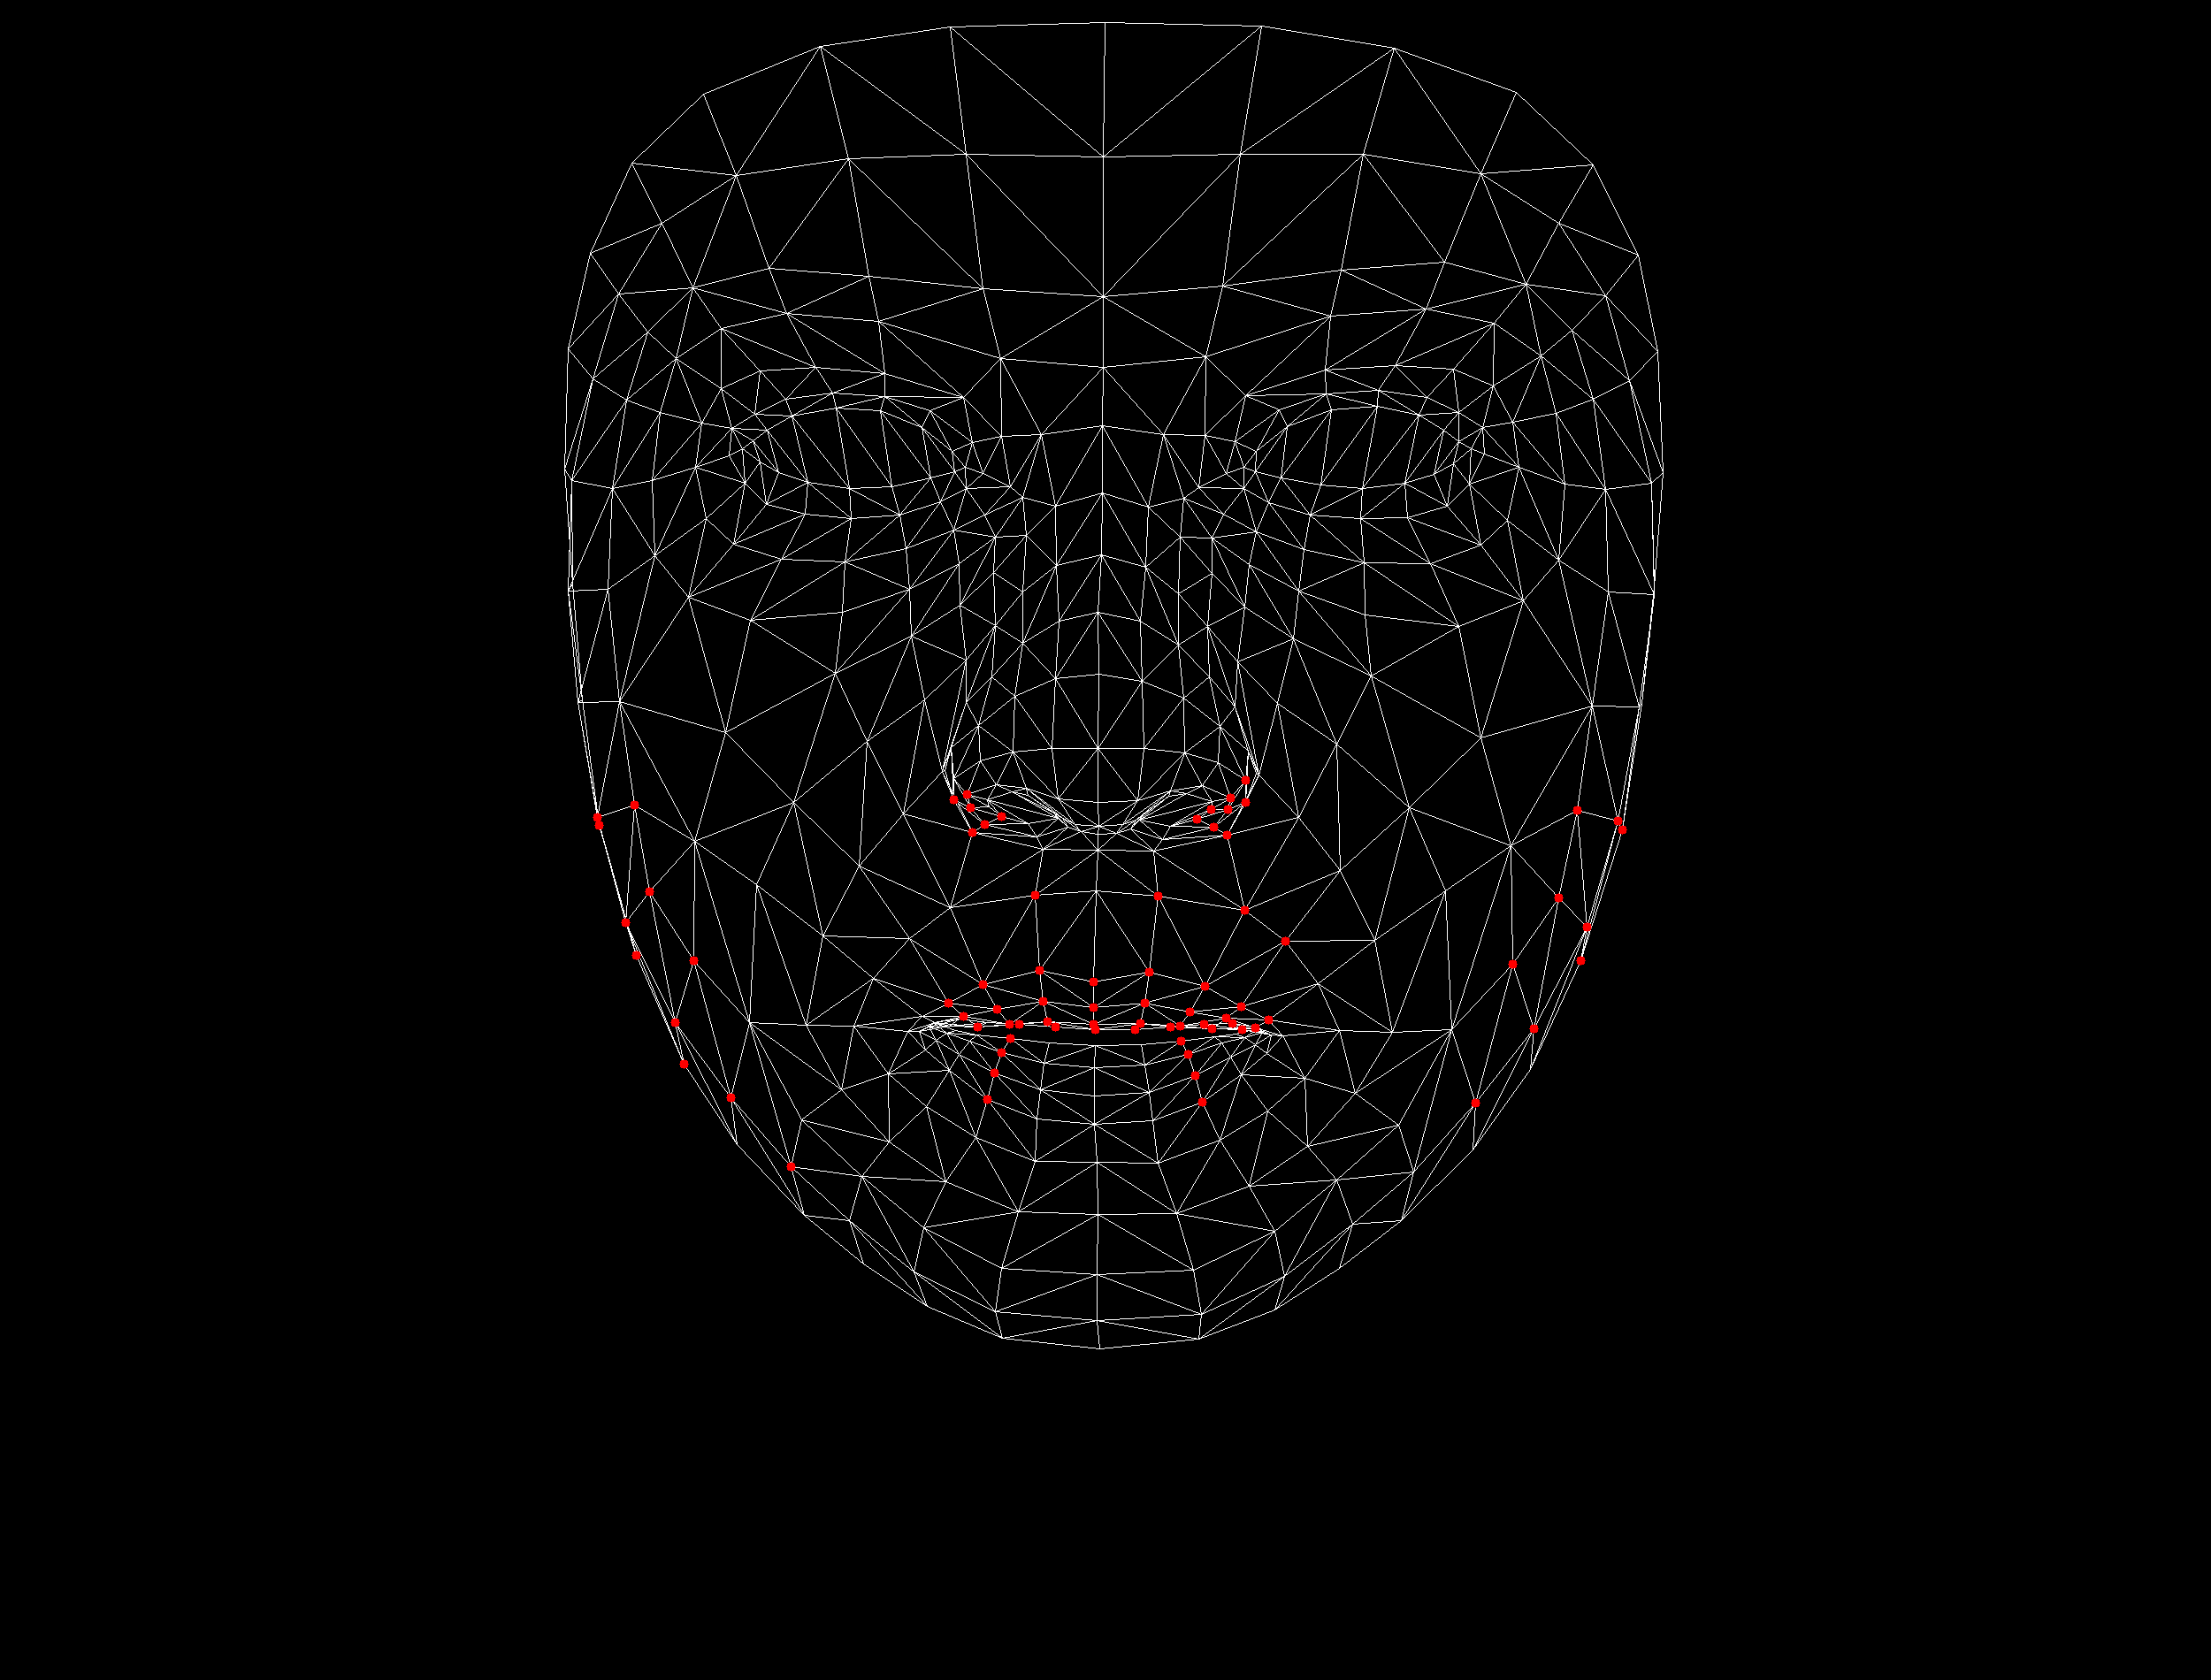
\includegraphics[width=0.5\textwidth]{images/pav_mask.png}

Com estes 77 pontos em mão, para cada máscara foi calculada a média deles, criando o arquivo masks\_means\_pav.csv
pav = points above average

\paragraph{Remoções do dataset}
\begin{itemize}
    \item {Usuário 06644: Não fez todas as capturas}
\end{itemize}



\subsubsection{Experimento 3 - Visualisação dos Dados}
\paragraph{Gráfcos de PseudoClustering}\mbox{}\\
\paragraph{Analise da distribuição das distancias da segunda abordagem do experimento 2}\mbox{}\\
\paragraph{Cluster com Kmeans dos Pontos acima da Média (PAV)}\mbox{}\\
Como foram selecionados 77 pontos, houve uma sobrecarga de dados para fazer a analise. Então foi utilizada esta técnica de clusterização para reduzir a quantidade de dados. Os 77 pontos foram dividos em 6 grupos, mostrados na imagem abaixo
(tb n sei se é aqui que eu dvo colocar a img)
A relação ponto-grupo esta salvo no arquivo points\_above\_average.csv Para a execução dos testes na secção 04 será utilizada a média de cada de distância de cada ponto

\subparagraph{Expansão dos grupos}\mbox{}\\
Dois novos grupos serão adicionados para analise arbitrariamente para ser feita uma visualização da relação do tamanho do sorriso com a contração dos olhos, para verificar se o sorriso é, de fato verdadeiro. Esta nova relação de grupos está no arquivo points\_above\_average\_expanded.csv

\paragraph{Remoções do Dataset}\mbox{}\\
\begin{itemize}
    \item {02935: Não respondeu aos questionários}
\end{itemize}

\subsubsection{Experimento 4 - Cálculo de Correlações}
aqui eu vou escrever depois pq eu não anotei no github...
\subsubsection{Experimento 5 - Testes de Hipóteses}
\paragraph{pessoa com score mais alto em depressão tende a ter uma media maior das distancias da face neutra pra neutra media dos participantes}
isso aqui serviu p testar se os sorrisos eram verdadeiros
explicar que eu vou fazer o teste com o score bdi e o kmeans expandido pra pegar a contração do olho

\section{Resultados e Discussão}
\label{sec:resultados}

\subsection{Máscaras}
\subsubsection{Máscaras médas por expressão}\mbox{}\\
\subsubsection{Diferenças entre Supervisionado e Não SUpervisionado}\mbox{}\\
Notou-se que:
\begin{itemize}
    \item Na 05 (Alegria) foi mais comum rostos mais expressivos e com sorrisos maiores na captura \emph{não supervisionada} do que na supervisionada.
    \item Na 07 (Surpresa) aconteceu o oposto da 05, pois foi mais comum bocas com uma amplitude de abertura maior nas capturas \emph{supervisionadas} do que nas não supervisionadas
\end{itemize}

\subsubsection{Comparações entre máscaras médias supervisionadas e não supervisionadas}\mbox{}\\

A coluna da esquerda representa as mascaras não supervisionadas e a da direita as supervisionadas. A cada Bloco de imagem são apresentadas 4 imagens sendo duas máscaras "fantasmas" e duas de pontos médios.
A máscara fantasma apresenta os vestígios de todas as mascaras analisadas simultaneamente, reforçando os pixels onde as linhas mais aparecem.
A máscara de pontos médios apenas faz uma média das posições x,y de cada um dos landmarks da expressão e desenha uma máscara a partir disso.

COLOCAR AS IMAGENS AQUI


\subsubsection{Distância entre os pontos da expressão Neutra Não Supervisionada}\mbox{}\\

Aqui foram geradas visualizações das máscaras obtendo a distancia entre os landmarks da máscara média de uma dada expressão para a média da Neutra não supervisionada. E para gerar o heatmap foi pintado um triângulo com o valor médio dos 3 vértices que o compõem.

COLOCAR AS IMAGENS AQUI DA ESCALA DINAMICA (ACHO QUE AQUELA COR TA ÓTIMA)

\subsubsection{Grupos Faciais}\mbox{}\\
Como foi dito no item ?? foram separados 77 pontos cujas distâncias até seu correspondente na neutra NS são maiores que a média do restante de sua máscara.
Para obter estes pontos foram analisados os seguintes dados aqui representados em gráficos:

COLOCAR OS GRÁFICOS AQUI

E então foram separados nos seguintes pontos destacados em vermelho

COLOCAR A IMAGEM COM OS PONTOS DESTACADOS AQUI (NÃO COLOCAR ELA NO 3)

E conforme foi observado pelo bolsista, a quantidade de dados ainda era absurdamente grande, portanto foi necessário reduzir a quantidade de dados para aumentar a velocidade de processamento. Para tal foi utilizado o método de K-means para reduzir a quantidade de dados. Gerando os seguintes grupos de pontos

COLOCAR A IMAGEM DO KMEANS PADRÃO

\subsection{Correlações Mais Fortes}
Conforme foi discutido no item ?? os testes de correlação foram feitos utilizando os grupos faciais obtidos pelo método de clusterização Kmeans, e correlacionando-os com os scores dos questionários psiquiátricos descritos no item ??. (é seria legal descrever eles e colocar eles no apendice talvez, ou anexo sla)

Algumas correlações fortes foram encontradas, como a Beck Anxiety Inventory VERSUS Obsessive-Compulsive Inventory, contudo como este tipo de correlação entre scores dos questionários ja foi amplamente discutido na literatura, não foi dispendido tempo para analisá-los.

As melhores correlações obtidas foram:


\begin{itemize}
    \item Grupo 02 da Alegria não supervisionada VERSUS Adult Self-Report Scale (Hiperatividade)
    \begin{itemize}
        \item spearmanr
            \subitem pvalue = 0.0001702527593707
            \subitem rvalue = 0.2122881902011349
        \item pearsonr
            \subitem pvalue = 6.888895152022905e-05
            \subitem rvalue = 0.2244339895379587
    \end{itemize}
\item Grupo 02 da Alegria supervisionada VERSUS Adult Self-Report Scale (Hiperatividade)
    \begin{itemize}
        \item spearmanr
            \subitem pvalue = 0.0003732745538004
            \subitem rvalue = 0.2011662537681749
        \item pearsonr
            \subitem pvalue = 0.0043378892933926
            \subitem rvalue = 0.1618568566694145
    \end{itemize}
\end{itemize}


\subsection{Problema de Aquisição}

\subsubsection{Testes}\mbox{}\\

Para avaliar a hipótese de que um sorriso verdadeiro contrai os olhos e que pessoas com score alto no DBI não expressam sorrisos tão fortes, foi criado mais 2 grupos faciais arbitrários na mascara, apresentados abaixo:

COLOCAR KMEANS EXPANDIDO AQUI

Com isso, seria possível verificar a média de distância do grupo 5 com o grupo 6 e do grupo 1 com o grupo 7. Assim, seria esperado encontrar dados como o exemplo abaixo:

COLOCAR O GRAFICO esperado

Contudo o que foi encontrado foi:

COLOCAR UNS PRINTS E LINKS PROS HTML INTERATIVOS

E observando os gráficos nota-se que não condiz com o que era esperado, portanto pode-se inferir que a coleta criou este erro ou a premissa da hipótese era falsa.
Além disso, para a analise de expressões faciais é necessário que hajam vídeos da expressão surgindo e se dissipando (buscar referencia disso)
%\section{Atividades Relevantes Desenvolvidas pelo Bolsista}
\label{sec:atividades}

Participações em Congressos, Seminários, Cursos etc., trabalhos apresentados e publicados em eventos científicos

%\section{Dificuldades Encontradas}
\label{sec:dificuldades}

não relatar dificuldade pessoal, tal como a falta de conhecimento linguístico do bolsista

%\section{Cronograma de Execução}
\label{sec:cronograma}

%\section{Considerações <Parciais ou Finais>}
\label{sec:consideracoes}

%\section{Parecer do Orientador}


\noindent Recife, DD  de MMMMMMM  de 20AA 
\\[1.5cm]
----------------------------------------\\
Assinatura do Orientador\\
\\[1.5cm]
----------------------------------------\\
Assinatura do Aluno
\section{Conclusões}
\label{sec:conclusoes}
\renewcommand\refname{Referências Bibliográficas}
%\bibliographystyle{abntex2-alf}
\bibliographystyle{IEEEtran}
\bibliography{referencias.bib}
%\listoftodos

\end{document}